\documentclass[11pt,a4paper]{article}

\usepackage[margin=1in]{geometry}
\usepackage{amsmath,amssymb}
\usepackage{graphicx}
\usepackage{booktabs}
\usepackage{hyperref}
\usepackage{xcolor}
\usepackage{microtype}
\usepackage{setspace}
\setstretch{1.07}

\hypersetup{
  colorlinks=true,
  linkcolor=black,
  citecolor=blue!50!black,
  urlcolor=blue!60!black
}

\title{\textbf{DenoiseOpt:} Residual Scoring and Bi-Level\\
Meta-Learning for Wavetable Wrap Crackle}
\author{
  Julian~M.~Kleber\\
  ORCID: \href{https://orcid.org/0000-0001-5518-0932}{0000-0001-5518-0932}\\
  Email: \href{mailto:julian.m.kleber@gmail.com}{julian.m.kleber@gmail.com}\\[0.6em]
  \small
  Synth:
  \href{https://github.com/reeldemo/reelsynth}{github.com/reeldemo/reelsynth}\\
  Meta artifacts:
  \href{https://github.com/reeldemo/denoise-opt-meta}{github.com/reeldemo/denoise-opt-meta}
}
\date{18 July 2026 \\ \small Synced with denoise-opt-meta \texttt{paper/v2}}

\begin{document}
\maketitle

\begin{abstract}
Open wrap seams inject audible crackle under cyclic wavetable playback.
DenoiseOpt is a seam-local bake stack scored without paired clean labels.
The outer meta objective is a prolonged residual score $\in[0,1]$ (1~=~best):
tiled DenoiseOpt output vs an ideal multi-period reference (same seed, no
open-wrap). Nested unsupervised loss $L=(1-\mathcal{D})+\lambda(1-\mathcal{S})$
optimizes $\theta$/$\lambda$ inside each trial. Across 1500 trials, Meta Top~1
\texttt{evo\_explore\_515} reaches residual $\approx 0.824$ vs DualCosine
$\approx 0.698$ ($N{=}2000$). Canonical PDF and versioning:
\href{https://github.com/reeldemo/denoise-opt-meta}{denoise-opt-meta} \texttt{paper/v2/}.
\end{abstract}

\section{Pointer}
Full paper, figures, and reproduction commands live in the public meta repo.
This tree mirrors the latest residual figures for local builds.

\begin{verbatim}
cargo run -p reelsynth --release --bin bench_denoise_meta
python brand/artifacts/render_benchmark_matrix.py
\end{verbatim}

\begin{figure}[t]
\centering
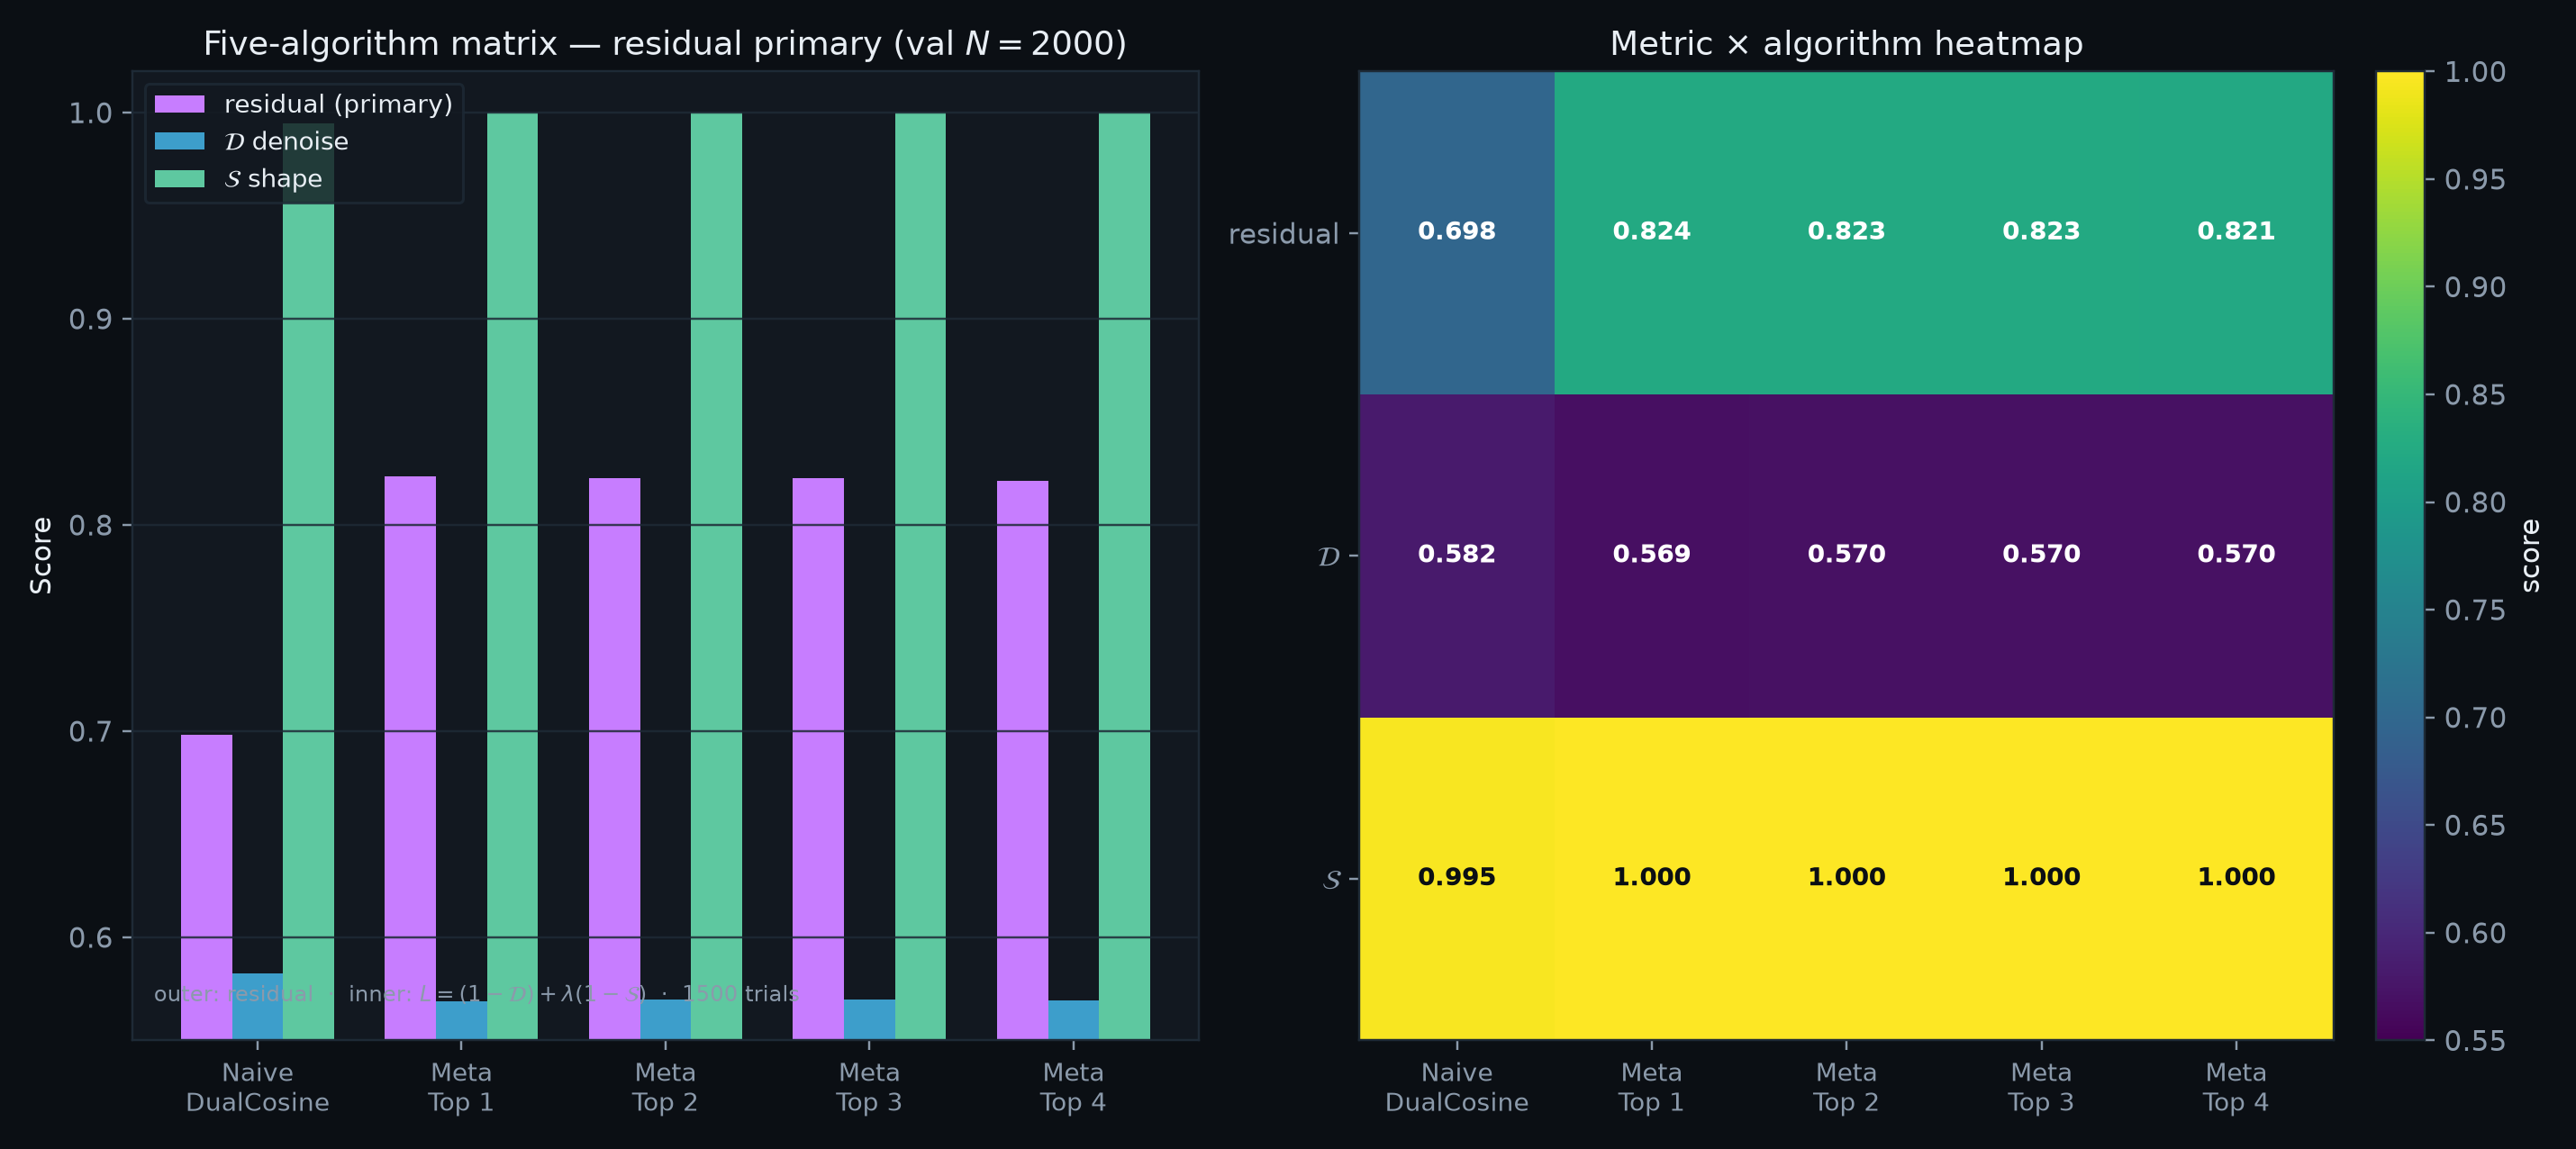
\includegraphics[width=\linewidth]{figures/fig_benchmark_matrix.png}
\caption{Residual-primary five-algorithm matrix (val $N{=}2000$).}
\end{figure}

\begin{table}[t]
\centering
\caption{Headline residual scores.}
\begin{tabular}{lcc}
\toprule
Algorithm & Residual & $Q$ \\
\midrule
Naive DualCosine & 0.698 & 0.789 \\
Meta Top~1 (\texttt{evo\_explore\_515}) & 0.824 & 0.784 \\
\bottomrule
\end{tabular}
\end{table}

\end{document}
